\documentclass[11pt]{article}
\usepackage[margin=1in]{geometry}
\usepackage[T1]{fontenc}
\usepackage{newtxtext,newtxmath}
\usepackage{amsmath}
\usepackage{graphicx}
\usepackage{booktabs}
\usepackage{caption}
\usepackage{flafter}  % floats never appear before the place they are defined
\usepackage{xcolor}
\usepackage[numbers,sort&compress]{natbib}
\usepackage[colorlinks=true,linkcolor=black,citecolor=black,urlcolor=black]{hyperref}

\captionsetup{font=small,labelfont=bf}
\setlength{\parskip}{0.35em}
\setlength{\parindent}{0pt}

% Every number quoted from the experiments is a macro written by `python -m e1.paper`
% (see generated/numbers.tex), so the text follows the data when seeds are added.
% Generated by `python -m e1.paper`. Do not edit; rerun instead.
\newcommand{\GapSmallAdamw}{0.025}
\newcommand{\GapSmallMuon}{0.046}
\newcommand{\GapSmallSgd}{0.026}
\newcommand{\GapTopAdamw}{2.5}
\newcommand{\GapTopMuon}{1.0}
\newcommand{\GapTopSgd}{2.1}
\newcommand{\IdExcessAdamw}{0.5--0.8}
\newcommand{\IdExcessMuon}{0.2--0.5}
\newcommand{\IdExcessSgd}{0.5--0.7}
\newcommand{\LevelAdamwSeedA}{11.10}
\newcommand{\LevelAdamwSeedB}{10.92}
\newcommand{\LevelMuonSeedA}{11.66}
\newcommand{\LevelMuonSeedB}{12.06}
\newcommand{\LevelSgdSeedA}{11.35}
\newcommand{\LevelSgdSeedB}{11.40}
\newcommand{\LevelShiftSeedAMuon}{+0.56}
\newcommand{\LevelShiftSeedASgd}{+0.25}
\newcommand{\LevelShiftSeedBMuon}{+1.14}
\newcommand{\LevelShiftSeedBSgd}{+0.47}
\newcommand{\LevelTau}{0.005}
\newcommand{\MemSpeedMuon}{5.0}
\newcommand{\MemSpeedSgd}{1.4}
\newcommand{\MstarAdamw}{11.47}
\newcommand{\MstarAdamwHi}{11.75}
\newcommand{\MstarAdamwLo}{11.39}
\newcommand{\MstarAdamwSeedA}{11.75}
\newcommand{\MstarAdamwSeedB}{11.39}
\newcommand{\MstarMuon}{not bracketed}
\newcommand{\MstarMuonHi}{14.52}
\newcommand{\MstarMuonLo}{11.92}
\newcommand{\MstarMuonSeedA}{11.92}
\newcommand{\MstarMuonSeedB}{14.52}
\newcommand{\MstarSgd}{10.90}
\newcommand{\MstarSgdHi}{11.50}
\newcommand{\MstarSgdLo}{10.72}
\newcommand{\MstarSgdSeedA}{11.50}
\newcommand{\MstarSgdSeedB}{10.72}
\newcommand{\NRuns}{108}
\newcommand{\NSeeds}{2}
\newcommand{\NuAdamw}{--}
\newcommand{\NuAdamwLarge}{--}
\newcommand{\NuMuon}{1.58}
\newcommand{\NuMuonLarge}{1.40}
\newcommand{\NuSgd}{--}
\newcommand{\NuSgdLarge}{1.17}
\newcommand{\OnsetPct}{5}
\newcommand{\PhiSmallAdamw}{11}
\newcommand{\PhiSmallLargeAdamw}{19}
\newcommand{\PhiSmallLargeMuon}{32}
\newcommand{\PhiSmallLargeSgd}{19}
\newcommand{\PhiSmallMuon}{28}
\newcommand{\PhiSmallSgd}{9}
\newcommand{\PredShiftLargeMuon}{+1.0}
\newcommand{\PredShiftLargeSgd}{+1.2}
\newcommand{\PredShiftMuon}{+1.1}
\newcommand{\PredShiftSgd}{+0.5}
\newcommand{\ProbeIdAdamw}{1.06}
\newcommand{\ProbeIdMuon}{1.03}
\newcommand{\ProbeIdSgd}{1.05}
\newcommand{\ProbeInputThirdAdamw}{1.04--2.32}
\newcommand{\ProbeInputThirdMuon}{1.03--1.05}
\newcommand{\ProbeInputThirdSgd}{1.09--1.13}
\newcommand{\ProbeInputThreeAdamw}{34.24--57.48}
\newcommand{\ProbeInputThreeMuon}{28.39--190.42}
\newcommand{\ProbeInputThreeSgd}{19.25--48.94}
\newcommand{\ProbeQueryFourAdamw}{3.22--6.20}
\newcommand{\ProbeQueryFourMuon}{2.95--13.00}
\newcommand{\ProbeQueryFourSgd}{2.82--3.79}
\newcommand{\ProbeQuerySixteenAdamw}{25}
\newcommand{\ProbeQuerySixteenMuon}{25}
\newcommand{\ProbeQuerySixteenSgd}{23}
\newcommand{\ProbeSkewAdamw}{5.04--8.31}
\newcommand{\ProbeSkewMuon}{3.80--14.41}
\newcommand{\ProbeSkewSgd}{1.76--26.99}
\newcommand{\ProbeZero}{27}
\newcommand{\ReboundPct}{10}
\newcommand{\RegSpeedMuon}{1.5}
\newcommand{\RegSpeedSgd}{2.5}
\newcommand{\RunHours}{193}
\newcommand{\SNHighAdamw}{8}
\newcommand{\SNHighMuon}{8}
\newcommand{\SNHighSgd}{8}
\newcommand{\SNLowAdamw}{8}
\newcommand{\SNLowMuon}{8}
\newcommand{\SNLowSgd}{8}
\newcommand{\SNegHighAdamw}{8}
\newcommand{\SNegHighMuon}{2}
\newcommand{\SNegHighSgd}{5}
\newcommand{\SPosLowAdamw}{8}
\newcommand{\SPosLowMuon}{8}
\newcommand{\SPosLowSgd}{7}
\newcommand{\SeedA}{42}
\newcommand{\SeedB}{755}
\newcommand{\ShiftPooledMuon}{--}
\newcommand{\ShiftPooledSgd}{-0.57}
\newcommand{\ShiftSeedAMuon}{+0.17}
\newcommand{\ShiftSeedASgd}{-0.25}
\newcommand{\ShiftSeedBMuon}{+3.12}
\newcommand{\ShiftSeedBSgd}{-0.68}
\newcommand{\StepMinAdamw}{118/88}
\newcommand{\StepMinMuon}{20/21}
\newcommand{\StepMinSgd}{82/116}
\newcommand{\TmemReached}{0}
\newcommand{\TonAdamw}{272/306}
\newcommand{\TonMuon}{62/54}
\newcommand{\TonSgd}{432/382}
\newcommand{\TregAdamw}{14/20}
\newcommand{\TregMuon}{11/11}
\newcommand{\TregSgd}{42/43}


% \input is not expandable, which breaks booktabs rules after an included table body.
\makeatletter\newcommand{\tabinput}[1]{\@@input #1 }\makeatother
\newcommand{\todo}[1]{\textcolor{red}{[TODO: #1]}}
\newcommand{\Mstar}{M^{*}}
\newcommand{\dridge}{\Delta_{\mathrm{ridge}}}
\newcommand{\treg}{t_{\mathrm{reg}}}
\newcommand{\tmem}{t_{\mathrm{mem}}}
\newcommand{\ton}{t_{\mathrm{on}}}

\title{\vspace{-1.5em}How Does the Optimizer Shape Generalization in In-Context Regression?}
\author{Arihant Kaul \qquad Phil Liu \qquad Nayan Ramakrishnan \qquad Juan Calderon\\[0.3em]
\normalsize UC Berkeley, CS 182}
\date{\small Draft of 24 November 2026. Results from \NSeeds{} of 4 planned seeds; see Section~\ref{sec:limits} for what is not yet run.}

\begin{document}
\maketitle

\begin{abstract}
\noindent Transformers trained on in-context linear regression with a fixed pool of $M$ tasks behave like ridge regression, and so generalize to new tasks, only when $M$ exceeds a task-diversity threshold $\Mstar$. The threshold has been measured almost only under Adam. We train the 4-layer model of Ravent\'os et al.\ with AdamW, Muon and SGD on nine pool sizes, two batch sizes and \NSeeds{} seeds (\NRuns{} runs of 500{,}000 steps). Under AdamW we recover the published threshold ($\log_2 \Mstar = \MstarAdamw$ against $11.5$). Under Muon the transition sits higher: the batch-size statistic that locates $\Mstar$ stays positive in most runs up to $2^{13}$, and two other measures of the transition put it between half a doubling and two doublings of $M$ above AdamW's. SGD's threshold cannot be told apart from AdamW's. The Muon shift agrees in sign and rough size with a two-clock argument: Muon reaches ridge-level error \RegSpeedMuon{} times sooner than AdamW but begins to memorize the pool \MemSpeedMuon{} times sooner. No run came closer to dMMSE than to ridge in 500{,}000 steps. On off-distribution prompts, models at near-equal in-distribution error differ by optimizer no more than they differ between runs of one optimizer, with one exception: when all inputs are shrunk, Muon stays within 5\% of ridge in every run. Learning rates for Muon and SGD are not yet tuned and the learning-rate control is not yet run, so the optimizer effect is not yet separated from a learning-rate effect.
\end{abstract}

\section{Introduction}

A transformer trained on sequences $(x_1, y_1, \dots, x_K, y_K)$ with $y_k = w^\top x_k + \varepsilon_k$ can learn to predict $y_k$ from the examples before it, with no weight update at test time \citep{garg2022}. \citet{raventos2023} showed that what it learns depends on how many distinct tasks $w$ it saw. With a fixed pool of $M$ tasks, the predictor that minimizes training loss is the Bayes estimator under a uniform prior on the pool (dMMSE), which memorizes the pool and fails on new tasks. Above a threshold $\Mstar$ (about $2^{11.5}$ for a 4-layer model) trained transformers instead track ridge regression, the Bayes estimator under the Gaussian prior the pool was drawn from, and generalize.

Which solution wins is a property of training, not of the loss alone. \citet{nguyen2025} describe it as a race: the model generalizes if it learns the in-context algorithm before it memorizes the task set. \citet{carroll2025} show that models just below the threshold pass through ridge on the way to dMMSE, and \citet{wurgaft2025} that the time to memorize grows faster than linearly in $M$. All of this was measured under Adam (or, in \citet{nguyen2025}, SGD on a one-layer classifier).

The optimizer is an obvious thing to vary in a race. Muon \citep{jordan2024} replaces the momentum of each hidden weight matrix by its nearest semi-orthogonal matrix, and recent work disagrees on what that does to generalization. \citet{dragutinovic2026} prove that spectral descent loses the simplicity bias of gradient descent, and \citet{liu2026} report that Muon leans toward rote memorization relative to AdamW; \citet{ruan2026} instead find Muon's features more robust and transferable. \citet{chen2026} show that Muon bounds weight spectral norms only with weight decay on.

We ask three questions.
\begin{description}\setlength{\itemsep}{0pt}
\item[Q1.] Does the choice among SGD, AdamW and Muon move $\Mstar$, and by more than retuning the learning rate does?
\item[Q2.] Is the shift predicted by two separately measured clocks: how fast an optimizer learns regression and how fast it memorizes \citep{nguyen2025}?
\item[Q3.] At equal in-distribution loss, do optimizers differ on the off-distribution prompts of \citet{garg2022}?
\end{description}

\textbf{Status of the answers.} This draft reports the threshold grid for \NSeeds{} seeds and analyses that need no further training. Table~\ref{tab:status} lists what was planned and what was run. In short: Q1 has an answer for the direction of the Muon shift but not for the comparison with learning-rate retuning; Q2 has a qualitative answer from stand-in clocks; Q3 has an answer at the end of training only.

\begin{table}[!htb]
\centering\small
\caption{Planned experiments and what this draft contains.}
\label{tab:status}
\begin{tabular}{@{}p{0.2\linewidth}p{0.3\linewidth}p{0.43\linewidth}@{}}
\toprule
Experiment & Planned & In this draft \\
\midrule
E1 threshold grid & 9 pool sizes, 3 optimizers, 2 batch sizes, 4 seeds & \NSeeds{} seeds, all \NRuns{} runs complete (Sections~\ref{sec:q1}--\ref{sec:dynamics}) \\
\addlinespace
E2 clocks & fresh-task runs, 10 seeds per optimizer & not run; clocks read from the E1 logs (Section~\ref{sec:q2}) \\
\addlinespace
E3a learning-rate control & $\Mstar$ at half and double the learning rate & not run \\
\addlinespace
E3b weight decay & AdamW and Muon with weight decay & not run \\
\addlinespace
E3c longer training & four times longer near threshold & not run \\
\addlinespace
E4 off-distribution probes & evaluation on fresh-task checkpoints through training & final weights at $M = 2^{15}$ only (Section~\ref{sec:q3}) \\
\bottomrule
\end{tabular}
\end{table}

\section{Setup}
\label{sec:setup}

\textbf{Task and model.} We use the testbed of \citet{raventos2023}: input dimension $D = 8$, $K = 16$ in-context examples, label noise variance $\sigma^2 = 0.25$. Each seed draws a pool of task vectors $w^{(i)} \sim \mathcal{N}(0, I_D)$ once; a run with pool size $M$ uses the first $M$ of them. Each training sequence samples a task from the pool, inputs $x_k \sim \mathcal{N}(0, I_D)$ and targets $y_k = w^{(i)\top} x_k + \varepsilon_k$. The model is a 4-layer GPT-2-style transformer of width 64 with 2 heads, trained with squared error on every position for 500{,}000 steps. The learning rate rises linearly to its peak at step 250{,}000 and falls linearly to zero, as in the reference code. Weight decay is zero throughout.

\textbf{Optimizers.} AdamW uses peak learning rate $10^{-3}$, the reference value for Adam in \citet{raventos2023}. Muon (Nesterov momentum 0.95) is applied to the two-dimensional weight matrices inside the transformer blocks with peak learning rate $5 \times 10^{-3}$; all other parameters use AdamW at $10^{-3}$. SGD uses momentum 0.9 and peak learning rate $0.1$. Only AdamW's value is a tuned reference. Muon's is the best of three values in a 20{,}000-step check on one seed. SGD's is untuned: in the same check it learned nothing at $0.1$ or below and diverged at $0.3$, and it does learn at $0.1$ over the full run. The proposal called for tuning each optimizer as in \citet{wen2026}; that has not been done.

\textbf{Grid.} $M \in \{2^{9}, 2^{10}, 2^{10.5}, 2^{11}, 2^{11.5}, 2^{12}, 2^{12.5}, 2^{13}, 2^{15}\}$, three optimizers, batch sizes 256 and 512 at the same number of steps, seeds \SeedA{} and \SeedB{}: \NRuns{} runs. Within a seed all runs share the pool, the initial weights and the evaluation prompts.

\textbf{Measures.} Following \citet{raventos2023}, the distance between the model $f_\theta$ and a reference predictor is
\[
\Delta_{\mathrm{ref}} \;=\; \mathbb{E}\Big[\tfrac{1}{KD} \textstyle\sum_{k} \big(f_\theta(S_k) - \hat{y}^{\mathrm{ref}}_k\big)^2\Big],
\]
where $S_k$ is the prompt up to $x_k$ and the reference is ridge (with $\lambda = \sigma^2$) or dMMSE, both in closed form. We evaluate on 8{,}192 fixed prompts with new tasks and 8{,}192 with pool tasks, every 1{,}000 steps.

\textbf{Locating the threshold.} In \citet{raventos2023}, more sequences per task push a model toward dMMSE below $\Mstar$ and toward ridge above it. We therefore define
\[
s(M) \;=\; \dridge^{\mathrm{new}}(M;\ \text{batch } 512) \;-\; \dridge^{\mathrm{new}}(M;\ \text{batch } 256),
\]
paired by seed, and take $\Mstar$ as the pool size at which $s$ changes from positive to negative, interpolated linearly in $\log_2 M$. We report the crossing of the seed-averaged curve, the crossing for each seed, and the range of crossings over resampled sets of seeds. With two seeds that range is only the span between the two seeds and their average; it is not a confidence interval.

We add three measures that were not in the proposal, because the planned single-run readout (the $M$ at which a model is equally far from both references on pool tasks) turned out to be empty: no run came closer to dMMSE than to ridge.
\begin{itemize}\setlength{\itemsep}{0pt}
\item \emph{Level crossing} $M_\tau$: the pool size beyond which $\dridge^{\mathrm{new}}$ at the end of training stays below $\tau = \LevelTau$ (batch 256).
\item \emph{Leaving ridge}: a run left ridge if $\dridge^{\mathrm{new}}$ ended more than \ReboundPct\% above its minimum during training. We report the largest pool size at which this happened.
\item \emph{Memorized fraction} $\varphi = (L_{\mathrm{ridge}} - L_{\theta}) / (L_{\mathrm{ridge}} - L_{\mathrm{dMMSE}})$, with $L$ the error on pool tasks against the noiseless target. $\varphi = 0$ is ridge and $\varphi = 1$ is dMMSE. Ridge is Bayes-optimal for tasks drawn from the Gaussian prior, so $\varphi > 0$ requires knowledge of the pool.
\end{itemize}

\section{Results}

\subsection{Q1: the threshold under each optimizer}
\label{sec:q1}

\begin{figure}[t]
\centering
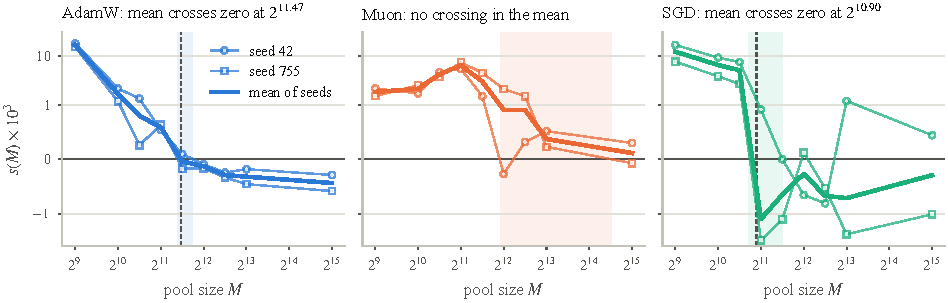
\includegraphics[width=\linewidth]{figures/fig_crossover.pdf}
\caption{The batch-size statistic $s(M)$ for each optimizer. Positive values mean that doubling the batch moved the model away from ridge on new tasks. Thin lines are seeds, the thick line their mean. The dashed line marks the crossing of the mean and the shaded band the range of crossings over resampled seeds. The vertical axis is linear between $-1$ and $1$ and logarithmic outside.}
\label{fig:crossover}
\end{figure}

\begin{table}[!htb]
\centering\small
\caption{Where the transition sits, by three measures, in $\log_2 M$. \emph{Batch-size crossover} is the proposal's definition of $\Mstar$; the range is over resampled seeds. \emph{LR status} says how the learning rate was chosen. $M_\tau$ and the last column (seed \SeedA{} / seed \SeedB) are defined in Section~\ref{sec:setup} and use batch 256. $^\dagger$The curve crosses zero more than once; the lowest crossing is shown.}
\label{tab:thresholds}
\setlength{\tabcolsep}{4.5pt}\begin{tabular}{@{}llcccccc@{}}
\toprule
 & & \multicolumn{3}{c}{Batch-size crossover $\log_2 \Mstar$} & \multicolumn{2}{c}{Level crossing $\log_2 M_\tau$} & Largest $M$ that \\
\cmidrule(lr){3-5}\cmidrule(lr){6-7}
Optimizer & LR status & seed \SeedA & seed \SeedB & pooled (range) & seed \SeedA & seed \SeedB & left ridge \\
\midrule
\tabinput{generated/tab_thresholds.tex}
\bottomrule
\end{tabular}
\end{table}

\textbf{AdamW reproduces the published threshold.} $s(M)$ is positive in \SPosLowAdamw{} of \SNLowAdamw{} seed--pool pairs up to $2^{11}$ and negative in \SNegHighAdamw{} of \SNHighAdamw{} pairs from $2^{12}$ up (Figure~\ref{fig:crossover}). The pooled crossing is $\log_2 \Mstar = \MstarAdamw$, with seeds at \MstarAdamwSeedA{} and \MstarAdamwSeedB{}, against $11.5$ reported for Adam on this architecture \citep{raventos2023}. We read this as evidence that our PyTorch port and the batch-size statistic behave as intended.

\textbf{Under Muon the transition is higher, and the statistic does not pin it down.} $s(M)$ is negative in only \SNegHighMuon{} of \SNHighMuon{} pairs from $2^{12}$ up, where AdamW is negative in all of them. The seed-averaged curve never crosses zero inside the grid. One seed crosses at \MstarMuonSeedA{}, through a single negative value at $2^{12}$ that is followed by positive ones; the other crosses at \MstarMuonSeedB{}. The other two measures agree on the direction. The level crossing is $\LevelShiftSeedAMuon$ and $\LevelShiftSeedBMuon$ doublings above AdamW's in the two seeds. Runs left ridge up to $2^{10.5}$ under Muon in both seeds and only at $2^{9}$ under AdamW, which puts that boundary between half a doubling and two doublings higher.

\textbf{SGD cannot be told apart from AdamW.} The pooled crossing is \MstarSgd{} ($\ShiftPooledSgd$ relative to AdamW), but the seeds give \MstarSgdSeedA{} and \MstarSgdSeedB{}, the second seed crosses zero more than once, and above $2^{12}$ the statistic takes both signs, at magnitudes up to several times AdamW's. The level crossing has the opposite sign ($\LevelShiftSeedASgd$ and $\LevelShiftSeedBSgd$).

\textbf{The proposal's decision rule.} We said a shift would count only if $|\Delta \log_2 \Mstar|$ exceeds both 0.5 and the spread across learning rates. The spread across learning rates is unmeasured (E3a), so no shift counts yet under that rule. Against the 0.5 bar alone, Muon's shift clears it on the level crossing in both seeds and on the batch-size crossover in one seed ($\ShiftSeedAMuon$ and $\ShiftSeedBMuon$); SGD's clears it in the pooled batch-size crossover and in one seed, with the opposite sign to its level crossing.

\begin{figure}[t]
\centering
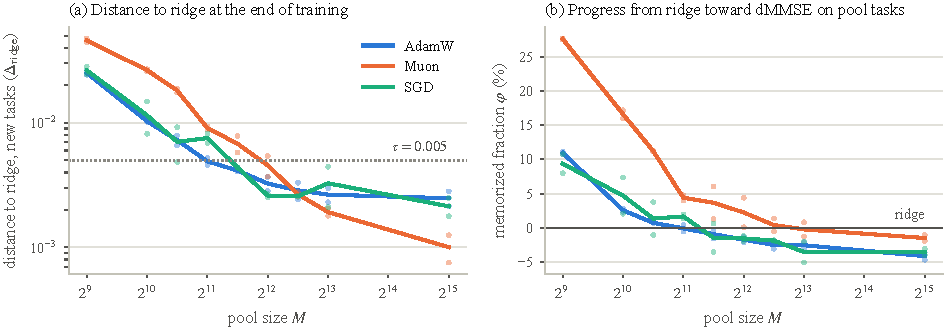
\includegraphics[width=\linewidth]{figures/fig_final_state.pdf}
\caption{State at the end of training, batch 256. Lines are means over seeds, dots are individual runs. (a) Distance to ridge on new tasks; the dotted line is the level $\tau$ used for $M_\tau$. (b) Memorized fraction on pool tasks. Muon is further from ridge than AdamW up to $2^{12}$ and closer to it from $2^{12.5}$.}
\label{fig:final}
\end{figure}

\subsection{What the runs do during training}
\label{sec:dynamics}

\begin{figure}[t]
\centering
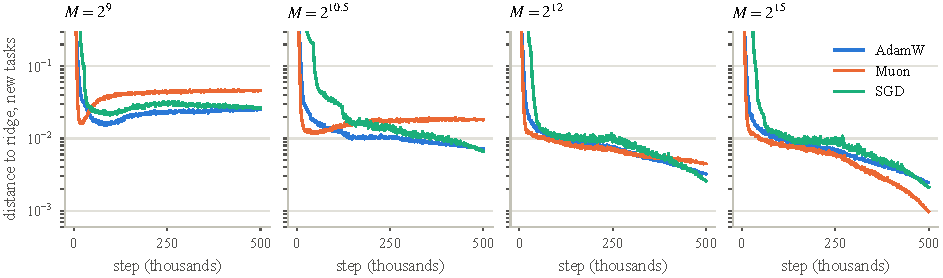
\includegraphics[width=\linewidth]{figures/fig_dynamics.pdf}
\caption{Distance to ridge on new tasks through training at four pool sizes (batch 256, geometric mean over seeds). At small pools every optimizer approaches ridge and then leaves it; Muon turns earliest and goes furthest. At $2^{15}$ Muon ends closest to ridge.}
\label{fig:dynamics}
\end{figure}

\textbf{Small pools pass through ridge and leave it.} At $M = 2^{9}$ every run approaches ridge and then moves away (Figure~\ref{fig:dynamics}), the transient described by \citet{carroll2025}. The distance to ridge is smallest at step \StepMinMuon{} thousand under Muon (seeds \SeedA{} and \SeedB), \StepMinAdamw{} thousand under AdamW and \StepMinSgd{} thousand under SGD.

\textbf{Muon sharpens both ends.} At the end of training (Figure~\ref{fig:final}a) Muon is the furthest from ridge at small pools ($\dridge^{\mathrm{new}} = \GapSmallMuon$ at $2^{9}$, against \GapSmallAdamw{} for AdamW and \GapSmallSgd{} for SGD) and the closest at the largest pool ($\GapTopMuon \times 10^{-3}$ at $2^{15}$, against $\GapTopAdamw \times 10^{-3}$ and $\GapTopSgd \times 10^{-3}$). The two curves cross between $2^{12}$ and $2^{12.5}$.

\textbf{No run memorized the pool.} The proposal's memorization clock $\tmem$, the first step at which predictions on pool tasks are closer to dMMSE than to ridge, was reached in \TmemReached{} of \NRuns{} runs. At $2^{9}$ and batch 256 the memorized fraction at the end of training is \PhiSmallAdamw\% under AdamW, \PhiSmallMuon\% under Muon and \PhiSmallSgd\% under SGD (Figure~\ref{fig:final}b); at batch 512 it is \PhiSmallLargeAdamw\%, \PhiSmallLargeMuon\% and \PhiSmallLargeSgd\%. At the small pools it is at its highest at the last evaluation, so it had not levelled off when the learning rate reached zero. The runs below threshold in our grid are therefore partial memorizers at 500{,}000 steps, and ``below threshold'' in this paper means moving away from ridge, not having arrived at dMMSE.

\subsection{Q2: two clocks}
\label{sec:q2}

\begin{figure}[t]
\centering
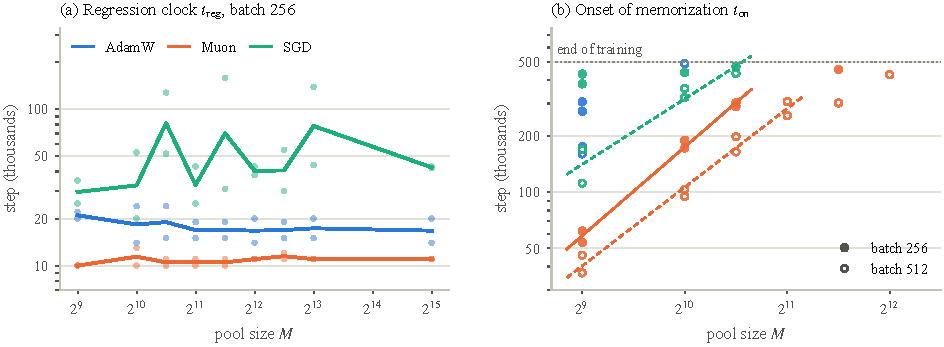
\includegraphics[width=\linewidth]{figures/fig_clocks.pdf}
\caption{The two clocks, read from the E1 logs. (a) First step at which new-task error is within 10\% of ridge's, at every pool size; lines are geometric means over seeds. (b) First step from which the memorized fraction stays at or above \OnsetPct\%. Points are runs; runs that never reached the level are absent. Lines are power-law fits over the pool sizes at which both seeds reached it (solid: batch 256, dashed: batch 512).}
\label{fig:clocks}
\end{figure}

\begin{table}[!htb]
\centering\small
\caption{Clocks by optimizer and batch size. $\treg$ is read at $M = 2^{15}$ and $\ton$ at $M = 2^{9}$, in thousands of steps for seeds \SeedA{} / \SeedB{}; ratios are geometric means relative to AdamW at the same batch size. $\varphi$ is the memorized fraction at the end of training at $2^{9}$. $\nu$ is the exponent of $\ton \propto M^{\nu}$, with the number of pool sizes in the fit.}
\label{tab:clocks}
\begin{tabular}{@{}lccccccc@{}}
\toprule
Optimizer & Batch & $\treg$ & ratio & $\ton$ & ratio & $\varphi$ (\%) & $\nu$ (pool sizes) \\
\midrule
\tabinput{generated/tab_clocks.tex}
\bottomrule
\end{tabular}
\end{table}

The proposal planned to measure a regression clock $\treg$ on fresh-task runs and a memorization clock $\tmem(M)$ on runs below threshold, fit $\tmem = c M^{\nu}$, and predict $\hat{M}^{*} = (\kappa\, \treg / c)^{1/\nu}$ with $\kappa$ calibrated on AdamW. Neither clock is available in that form: fresh-task runs were not made, and $\tmem$ was never reached. We use two stand-ins from the E1 logs.

\textbf{Regression clock.} $\treg$ is the first logged step at which new-task error is within 10\% of ridge's, read at $M = 2^{15}$. Under AdamW and Muon it barely depends on $M$ (Figure~\ref{fig:clocks}a), so the largest pool is a fair substitute for fresh tasks. Muon reaches the mark at step \TregMuon{} thousand, AdamW at \TregAdamw{} thousand and SGD at \TregSgd{} thousand: Muon is \RegSpeedMuon{} times faster than AdamW and SGD \RegSpeedSgd{} times slower. Under SGD the clock varies widely across pool sizes and seeds, because SGD sits on plateaus of varying length.

\textbf{Onset of memorization.} $\ton(M)$ is the first step from which $\varphi$ stays at or above \OnsetPct\% for five consecutive evaluations. At $2^{9}$ and batch 256, Muon reaches it at step \TonMuon{} thousand, AdamW at \TonAdamw{} thousand and SGD at \TonSgd{} thousand: Muon is \MemSpeedMuon{} times faster than AdamW and SGD \MemSpeedSgd{} times slower. Where there are enough points to fit, the onset grows faster than linearly in $M$ ($\nu = \NuMuon$ and \NuMuonLarge{} for Muon at the two batch sizes, \NuSgdLarge{} for SGD at batch 512), in line with \citet{wurgaft2025}. AdamW reaches the onset at one pool size only, so it has no fit.

\textbf{Does the race predict the shift?} If the threshold is where $c M^{\nu} = \kappa\, \treg$ and $\kappa$ and $\nu$ are shared, then relative to AdamW
\[
\Delta \log_2 \Mstar \;=\; \frac{\Delta \log_2 \treg - \Delta \log_2 c}{\nu},
\]
and $\Delta \log_2 c$ equals $\Delta \log_2 \ton$ at a fixed pool size. Taking $\nu$ from the Muon fit, this gives $\PredShiftMuon$ doublings for Muon at batch 256 ($\PredShiftLargeMuon$ at batch 512): Muon speeds memorization much more than it speeds regression, so the threshold should rise by about one doubling. That agrees in sign with all three measures of Section~\ref{sec:q1} and in size with the level crossing ($\LevelShiftSeedAMuon$, $\LevelShiftSeedBMuon$). For SGD the same calculation gives $\PredShiftSgd$ ($\PredShiftLargeSgd$ at batch 512), which matches the sign of the level crossing but not of the batch-size crossover. So the answer to Q2 is: the race predicts the direction and rough size of the Muon shift; for SGD neither the prediction nor the measurement is firm enough to test it. This is a consistency check built on stand-in clocks and a borrowed exponent, not the calibrated prediction the proposal described.

\subsection{Q3: off-distribution prompts}
\label{sec:q3}

\begin{figure}[t]
\centering
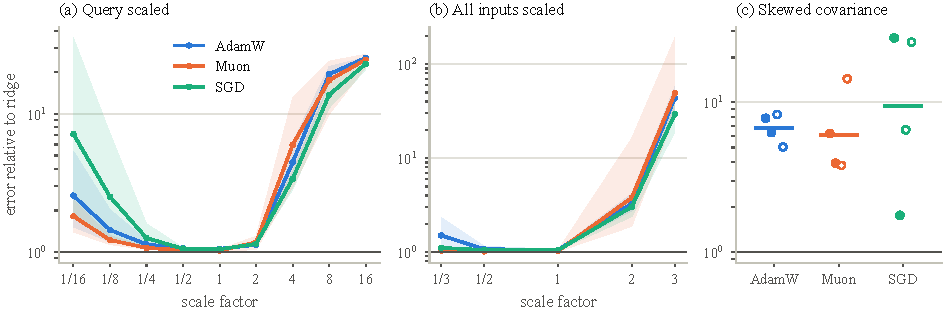
\includegraphics[width=\linewidth]{figures/fig_probes.pdf}
\caption{Error relative to ridge on shifted prompts, final weights at $M = 2^{15}$, at the last position (15 in-context examples). (a, b) Geometric mean over the four runs of each optimizer (two seeds, two batch sizes); bands span the smallest and largest run. (c) Each run under skewed input covariance (filled: batch 256, open: batch 512); bars are geometric means.}
\label{fig:probes}
\end{figure}

\begin{table}[!htb]
\centering\small
\caption{Error relative to ridge on the same prompts, final weights at $M = 2^{15}$: geometric mean over four runs (smallest--largest run). A value of 1 matches ridge.}
\label{tab:probes}
\begin{tabular}{@{}lccc@{}}
\toprule
Shift & AdamW & Muon & SGD \\
\midrule
\tabinput{generated/tab_probes.tex}
\bottomrule
\end{tabular}
\end{table}

We evaluate the final weights of the twelve $M = 2^{15}$ runs on the shifted prompts of \citet{garg2022}, with new tasks and the training noise level: the final input scaled by $1/16$ to $16$; all inputs scaled by $1/3$ to $3$; and inputs drawn from a Gaussian whose covariance has a random eigenbasis and eigenvalues proportional to $1/i^{2}$, normalized to the training input norm. Ridge with $\lambda = \sigma^{2}$ is the Bayes predictor on every one of these prompts, and we report the model's squared error divided by ridge's at the last position. These models are close to equal in-distribution: their new-task error exceeds ridge's by \IdExcessAdamw\% (AdamW), \IdExcessMuon\% (Muon) and \IdExcessSgd\% (SGD).

\textbf{Query scaling: no optimizer effect, as predicted.} All three optimizers degrade together (Figure~\ref{fig:probes}a). At a factor of 16 the ratio is \ProbeQuerySixteenAdamw{}, \ProbeQuerySixteenMuon{} and \ProbeQuerySixteenSgd{}; a predictor that always outputs zero would score \ProbeZero{}. The models' predictions have stopped growing with the query, which is what a final normalization layer that caps the output would produce. At intermediate factors the optimizers overlap run for run (at a factor of 4: \ProbeQueryFourAdamw{}, \ProbeQueryFourMuon{} and \ProbeQueryFourSgd{}).

\textbf{Input scaling and skew: no ordering, with one exception.} When all inputs are shrunk to a third, Muon stays at \ProbeInputThirdMuon{} times ridge in all four runs, against \ProbeInputThirdSgd{} for SGD and \ProbeInputThirdAdamw{} for AdamW. When inputs are enlarged or their covariance is skewed, every optimizer fails badly and the spread between runs of one optimizer is as large as the spread between optimizers (Table~\ref{tab:probes}); the single worst run on enlarged inputs is a Muon run. Under skewed covariance the four SGD runs alone span \ProbeSkewSgd{}.

So the answer to Q3 at the end of training is that we cannot reject the null hypothesis, except for shrunken inputs. The proposal's stronger test, tracing off-distribution error against in-distribution loss through training, needs intermediate checkpoints that these runs did not keep.

\section{Discussion}

Table~\ref{tab:hyp} sets the proposal's hypotheses against the evidence so far.

\textbf{What Muon changes.} Muon speeds up both clocks, and the memorization clock by more. The consequence is not that Muon generalizes worse or better overall, but that it moves the model further along whichever path the pool size selects in a fixed budget of steps: further toward the pool up to $2^{12}$, closer to ridge from $2^{12.5}$ (Figure~\ref{fig:final}a). This may be one way to reconcile the report that Muon leans toward memorization \citep{liu2026} with the report that its features transfer better \citep{ruan2026}: in our setting which one is observed depends on task diversity. We offer this as a conjecture; the present data cannot separate it from the simpler statement that Muon at our learning rate is a faster optimizer than AdamW at its reference rate.

\textbf{The batch-size statistic across optimizers.} The statistic was motivated by an observation made under Adam. Under AdamW it behaves as intended: large and positive at small pools, small and negative at large ones. Under Muon it peaks at $2^{11}$ rather than at the smallest pool, and at large pools its values are as small as AdamW's but of the opposite sign. Its sign at large pools may then reflect something other than the side of the threshold, for example that the batch-256 Muon runs are still improving toward ridge when training ends. We therefore lean on agreement between measures rather than on the crossover alone for Muon.

\begin{table}[!htb]
\centering\small
\caption{The proposal's hypotheses against the evidence so far.}
\label{tab:hyp}
\begin{tabular}{@{}p{0.36\linewidth}p{0.6\linewidth}@{}}
\toprule
Hypothesis & Evidence in this draft \\
\midrule
H1: $\Mstar_{\mathrm{SGD}} < \Mstar_{\mathrm{AdamW}} \le \Mstar_{\mathrm{Muon}}$, with the two-clock rule giving sign and rough size & Muon above AdamW: supported by three measures and by the clocks. SGD below AdamW: unresolved; measures disagree in sign. \\
\addlinespace
H2: weight decay lowers $\Mstar$, more for Muon & Not tested (E3b). \\
\addlinespace
H3: no optimizer effect under query scaling; Muon most robust under input scaling and skew & Query scaling: consistent. Input scaling: Muon most robust only for shrunken inputs. Skew and enlarged inputs: no ordering. \\
\addlinespace
Null: optimizer differences are no larger than those from retuning the learning rate & Cannot be assessed until E3a is run. \\
\bottomrule
\end{tabular}
\end{table}

\subsection{Limitations and remaining work}
\label{sec:limits}

\begin{itemize}\setlength{\itemsep}{1pt}
\item \textbf{Learning rate is confounded with optimizer.} Muon's learning rate is the best of three in a short check and SGD's is untuned. A higher effective learning rate would by itself speed both clocks. E3a (the threshold at half and double each learning rate) is the control that decides whether the Muon shift is an optimizer effect, and it is the first thing to run.
\item \textbf{Two seeds.} All ranges are spans over two seeds. Seeds 3 and 4 of the plan are not run. The Muon seeds disagree on the batch-size crossover by more than two doublings.
\item \textbf{Schedule.} The learning rate rises for the first half of training and falls to zero in the second. The clocks are therefore read at different learning rates: the regression clock early in warm-up, the memorization onset anywhere from warm-up into the decay. The end state is frozen by the schedule rather than converged; at small pools $\varphi$ was still rising at the end.
\item \textbf{Thresholds chosen after seeing the data.} The level $\tau$, the \ReboundPct\% rule for leaving ridge and the \OnsetPct\% onset level were chosen during analysis. The Muon level-crossing shift is positive at $\tau = 0.004$, $0.005$ and $0.008$ in both seeds and at both batch sizes, but none of these was fixed in advance.
\item \textbf{Stand-in clocks.} $\treg$ comes from pooled runs, $\ton$ replaces $\tmem$, and the exponent used for every optimizer comes from Muon. Fresh-task runs (E2) and longer runs near threshold (E3c) would give the clocks the proposal defined.
\item \textbf{Probes at one point.} Q3 is tested on final weights at $M = 2^{15}$, not on fresh-task models through training.
\item \textbf{Scale.} One architecture (4 layers, width 64), one task family, 8{,}192 evaluation prompts per set.
\end{itemize}

\section{Conclusion}

With two seeds and untuned learning rates for two of the three optimizers, the grid supports three statements. AdamW reproduces the published task-diversity threshold. Muon's transition sits higher, by an amount the planned statistic does not pin down and the other measures put at roughly one doubling of the pool, and this is the direction a race between a regression clock and a memorization clock predicts. Off the training distribution, optimizers at near-equal in-distribution error are not distinguishable beyond run-to-run variation, apart from Muon's robustness to shrunken inputs. Whether the Muon shift survives retuning the learning rate is the open question that decides Q1.

\section*{Contributions}
\todo{who did what}

\bibliographystyle{unsrtnat}
\bibliography{refs}

\appendix
\section{Full tables}

\begin{table}[h]
\centering\footnotesize
\caption{$s(M) \times 10^{3}$ for every optimizer, seed and pool size.}
\begin{tabular}{@{}llrrrrrrrrr@{}}
\toprule
\tabinput{generated/tab_s.tex}
\bottomrule
\end{tabular}
\end{table}

\begin{table}[h]
\centering\footnotesize
\caption{$\dridge^{\mathrm{new}} \times 10^{3}$ at the end of training, mean over seeds.}
\begin{tabular}{@{}llrrrrrrrrr@{}}
\toprule
\tabinput{generated/tab_gap.tex}
\bottomrule
\end{tabular}
\end{table}

\begin{table}[h]
\centering\footnotesize
\caption{Memorized fraction $\varphi$ (\%) at the end of training, mean over seeds. Negative values mean the model is still worse than ridge on pool tasks.}
\begin{tabular}{@{}llrrrrrrrrr@{}}
\toprule
\tabinput{generated/tab_phi.tex}
\bottomrule
\end{tabular}
\end{table}

\section{Implementation and differences from the proposal}

\begin{itemize}\setlength{\itemsep}{1pt}
\item \textbf{Code.} A PyTorch port of the reference JAX code of \citet{raventos2023}, not the JAX code itself: same architecture layout, initialization, loss and schedule; different random streams. Muon is PyTorch's implementation.
\item \textbf{Pools.} One pool of 32{,}768 tasks per seed, with smaller pools as prefixes, so pool sizes within a seed are nested.
\item \textbf{Evaluation.} 8{,}192 fixed prompts per set, against 1{,}048{,}576 in the reference code.
\item \textbf{Hardware.} Rented RTX 4090 and RTX 4070 Ti Super cards and one local RTX 4070 Ti; \RunHours{} run-hours of wall-clock time in total, with several runs sharing each card. Sixteen runs were stopped and continued from a checkpoint on a different card model. Inputs are generated on the CPU from seeded streams, so they are identical across machines; floating-point results are not bit-identical across card models.
\item \textbf{Reproduction.} From \texttt{code/}: \texttt{python -m e1.run\_seed -{}-seed 42 755} trains the grid; \texttt{python -m e1.aggregate}, \texttt{python -m e1.probes} and \texttt{python -m e1.paper} on the results folder produce every number, table and figure here.
\end{itemize}

\end{document}
